%iffalse
\let\negmedspace\undefined
\let\negthickspace\undefined
\documentclass[article,12pt,onecolumn]{IEEEtran}
\usepackage{cite}
\usepackage{amsmath,amssymb,amsfonts,amsthm}
\usepackage{algorithmic}
\usepackage{graphicx}
\usepackage{textcomp}
\usepackage{xcolor}
\graphicspath{{figs/}}
\usepackage{txfonts}
\usepackage{listings}
\usepackage{enumitem}
\usepackage{mathtools}
\usepackage{gensymb}
\usepackage{comment}
\usepackage[breaklinks=true]{hyperref}
\usepackage{tkz-euclide} 
\usepackage{listings}
\usepackage{gvv}
\def\inputGnumericTable{}                                 
\usepackage[utf8]{inputenc}                              
\usepackage{color}                                         
\usepackage{array}                                        
\usepackage{longtable}                                     
\usepackage{calc}                                          
\usepackage{multirow}                                      
\usepackage{hhline}                                        
\usepackage{ifthen}                                        
\usepackage{lscape}
\newtheorem{theorem}{Theorem}[section]
\newtheorem{problem}{Problem}
\newtheorem{proposition}{Proposition}[section]
\newtheorem{lemma}{Lemma}[section]
\newtheorem{corollary}[theorem]{Corollary}
\newtheorem{example}{Example}[section]
\newtheorem{definition}[problem]{Definition}
\newcommand{\BEQA}{\begin{eqnarray}}
\newcommand{\EEQA}{\end{eqnarray}}
\newcommand{\define}{\stackrel{\triangle}{=}}
\theoremstyle{remark}
\newtheorem{rem}{Remark}
\graphicspath{ {./Figures/} }
\usepackage{float} % For the [H] float option
\usepackage{textcomp}
\usepackage{multicol}

% --- myvec macro (wraps a bmatrix so your document keeps the same visual output
%     while using the requested \myvec command) ---

\begin{document}
\textbf{Question}\\[2pt]
Consider two points $P$ and $Q$ with position vectors
\[
\vec{P}=3\vec{a}-2\vec{b},
\qquad
\vec{Q}=\vec{a}+\vec{b}.
\]
Find the position vector of a point $R$ which divides the line joining $P$ and $Q$ in the ratio $2:1$,
\begin{enumerate}
    \item[(a)] internally, and
    \item[(b)] externally.
\end{enumerate}

\vspace{6pt}
\textbf{Solution}\\[2pt]

% Preamble:
% \usepackage{amsmath,amssymb}
\newcommand{\myvec}[1]{\begin{pmatrix}#1\end{pmatrix}}

\noindent We write the endpoints in matrix form:
\begin{equation}
\myvec{\vec P \;\; \vec Q}^{T}
=
\myvec{3 \;\; -2 \\[2pt] 1 \;\; 1}
\myvec{\vec a \\[2pt] \vec b}.
\label{eq:endpoints}
\end{equation}

\noindent \textbf{General section formulas (matrix form).}
For points \(\vec A,\vec B\) and ratio \(k:1\):
\begin{equation}
\vec R_{\text{int}}
=\frac{k\,\vec B+\vec A}{k+1}
=\frac{1}{k+1}\,[\,\vec A\;\;\vec B\,]\,
\myvec{1\\ k}.
\label{eq:int_general}
\end{equation}
\begin{equation}
\vec R_{\text{ext}}
=\frac{k\,\vec B-\vec A}{k-1}
=\frac{1}{k-1}\,[\,\vec A\;\;\vec B\,]\,
\myvec{-1\\ k}.
\label{eq:ext_general}
\end{equation}

\noindent \textbf{Internal division \(2:1\).}
Using \eqref{eq:int_general} with \(\vec A=\vec P,\ \vec B=\vec Q,\ k=2\),
\begin{equation}
\vec R_{\text{int}}
=\frac{1}{3}\,[\,\vec P\;\;\vec Q\,]\,
\myvec{1\\ 2}
=\myvec{\tfrac13 \;\; \tfrac23}\, \myvec{\vec P \;\; \vec Q}.
\label{eq:rint_def}
\end{equation}
Substitute \eqref{eq:endpoints} into \eqref{eq:rint_def}:
\begin{equation}
\vec R_{\text{int}}
=
\myvec{\tfrac13 \;\; \tfrac23}
\myvec{3 \;\; -2 \\[2pt] 1 \;\; 1}
\myvec{\vec a \\[2pt] \vec b}.
\label{eq:rint_sub}
\end{equation}
\begin{equation}
\boxed{\;\vec R_{\text{int}}=\tfrac{5}{3}\,\vec a\;}
\label{eq:rint_final}
\end{equation}

\noindent \textbf{External division \(2:1\).}
Using \eqref{eq:ext_general} with \(\vec A=\vec P,\ \vec B=\vec Q,\ k=2\),
\begin{equation}
\vec R_{\text{ext}}
=\,[\,\vec P\;\;\vec Q\,]\,
\myvec{-1\\ 2}
=\myvec{-1 \;\; 2}\,\myvec{\vec P \;\; \vec Q}.
\label{eq:rext_def}
\end{equation}
Substitute \eqref{eq:endpoints} into \eqref{eq:rext_def}:
\begin{equation}
\vec R_{\text{ext}}
=
\myvec{-1 \;\; 2}
\myvec{3 \;\; -2 \\[2pt] 1 \;\; 1}
\myvec{\vec a \\[2pt] \vec b}.
\label{eq:rext_sub}
\end{equation}
\begin{equation}
\boxed{\;\vec R_{\text{ext}}=-\,\vec a+4\,\vec b\;}
\label{eq:rext_final}
\end{equation}
\begin{figure}[H]
    \centering
    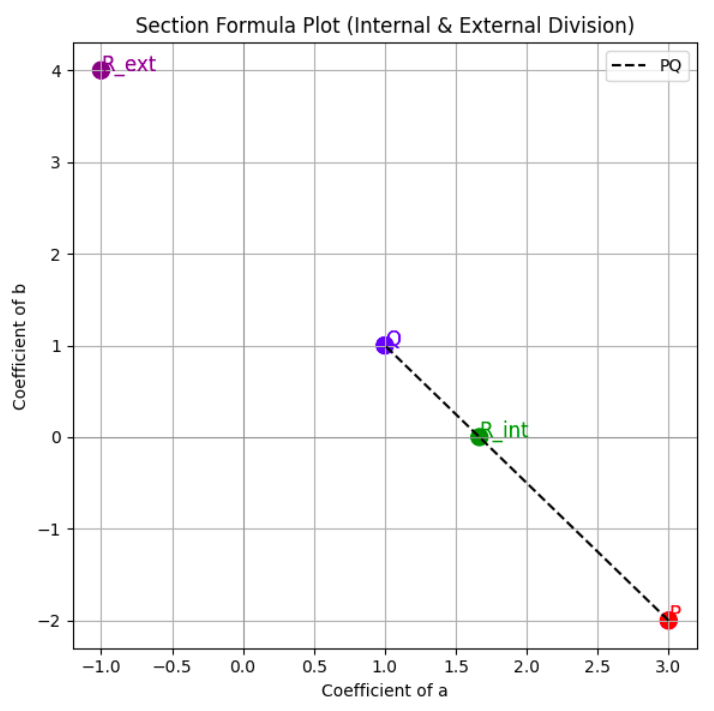
\includegraphics[width=\columnwidth]{figs/mg1plot.png}
\end{figure}

\end{document}
